\chapter{Applications to Neuromorphic Hardware}
\label{chapt:results}

The NEF and Nengo provide useful tools for programming recurrent spiking networks to implement algorithms formulated as dynamical systems.
The CPU backend is immensely useful for rapid prototyping of ideas, testing hypotheses, and experimenting with small-scale models on the order of a few thousand neurons.

\citep{knight2016}.
This section is taken from 


The accuracy of the system was evaluated by comparing the value at the output node of the network during recall with the output vector presented during training.
Both the SpiNNaker and reference simulator correctly recalled the output vectors with a consistent RMSE of approximately \num{0.2} at all scales.
However as Table~\ref{tab:results/memory_scale} shows, while the SpiNNaker simulations ran in real-time (\SI{0.25}{\second} per association), the time taken by the Nengo reference simulator grew quadratically -- over $150\times$ slower than real-time in the largest configuration.

\begin{table}
  \centering
  \caption{Simulation times on SpiNNaker and Nengo reference simulator}
  \label{tab:results/memory_scale}
\sisetup{table-number-alignment=right, table-figures-decimal=0}
\begin{tabular}{S S S r r}
  \toprule
  \multicolumn{2}{c}{Number of} & \multicolumn{2}{c}{Simulation time / minutes} \\
  {Associations} & {Neurons} & {SpiNNaker} & {Nengo Reference}\\
  \midrule
    250 & 12500 & 1.0 & 20.1 \\
    500 & 25000 & 2.1 & 75.5 \\
    1000 & 50000 & 4.2 & 309.0 \\
    2000 & 100000 & 8.3 & 1307.1 \\
  \bottomrule
\end{tabular}
\end{table}

The large number of afferent synapses associated with each neuron make simulating synaptic plasticity on SpiNNaker very computationally expensive.
In this paper we built on our previous work~\citep{mundy2015} to show that, by taking advantage of the factorable synaptic weight matrices used by the NEF and not simulating individual synapses, we can simulate both plastic and static spiking neural networks highly efficiently.
To demonstrate the benefits of this approach we implemented two biologically plausible learning rules on SpiNNaker and, using these, built a heteroassociative memory network that we proved to be capable of storing a human-scale semantic network.
By simulating this memory network at scales of up to \numprint{100000} neurons, we demonstrated that these two learning rules only reduce the number of neurons each SpiNNaker core can simulate by \SI{6}{\percent} and that by using SpiNNaker rather than a standard desktop PC, simulation times are reduced by over $150\times$.

\section{Integrator}
\label{sec:integrator}

\begin{figure}
  \centering
  \begin{subfigure}{.5\textwidth}
    \centering
    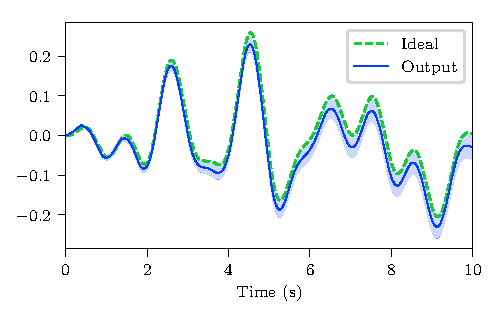
\includegraphics[width=\linewidth]{braindrop-integrator}
    \caption{Braindrop Chip}
    \label{fig:dn-braindrop}
  \end{subfigure}%
  \begin{subfigure}{.5\textwidth}
    \centering
    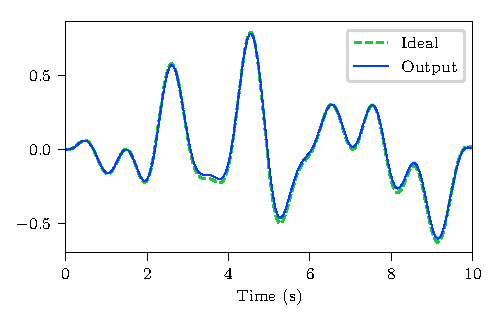
\includegraphics[width=\linewidth]{loihi-integrator}
    \caption{Loihi Emulator}
    \label{fig:dn-loihi}
  \end{subfigure}
  \caption{ \label{fig:integrator-neuromorphic}
    An integrator running on state-of-the-art neuromorphic hardware.
    The ideal solution is plotted against the mean's 95\% confidence interval, bootstrapped from $200$ trial simulations.
    (a)~Braindrop implementation, reproduced from \citet[][Figure~15]{braindrop2019}, using \numprint{1024} neurons. 
    (b)~Loihi Emulator (v0.4.0) implementation, using \numprint{256} neurons.
    See text for details.
  }
\end{figure}

The integrator, $\theta \dot{\V{x}}(t) = \V{u}(t)$, is a dynamical system used extensively by Spaun~\citep{eliasmith2012} and many other NEF and SPA models~\citep[][to name a few]{singh2004, trujillo2014a, rasmussen2017} for cognitive tasks involving working memory.
This system can persist information about the history of an input signal, starting from $t_0$ and extended indefinitely throughout time, as characterized by its solution:
$$\V{x}(t) = \V{x}(t_0) + \frac{1}{\theta} \int_{t'=t_0}^{t} \V{u}(t')\, dt' \text{.}$$
The parameter $\theta$ is a time-constant that controls how quickly the memory integrates new information.\footnote{
This parameter is useful for dimensional analysis, and when considering the transfer function, $\frac{\V{X}(s)}{\V{U}(s)} = \left( \theta s \right)^{-1}$.}
For example, beginning from an initial state of $\V{x}(t_0) = \V{0}$, if we hold the input constant at $\V{u}(t) = \V{v}$ for $\theta$ seconds ($t_0 < t \le t_0 + \theta$), and then clamp the input to $\V{u}(t) = \V{0}$ thereafter ($t > t_0 + \theta$), then $\V{x}(t) = \V{v}$ will ``store'' the vector $\V{v}$ indefinitely.
More generally, any finite set of nonlinear differential equations can be described as the integration of an input vector that is some nonlinear function of the state-vector---augmented to also include $\V{u}(t)$---as in $\theta \dot{\V{x}}(t) = \V{f}\left({\V{x}(t)}\right)$.
The nonlinearity $\V{f}(\cdot)$ may then be supported by a pool of neurons encoding the state-vector, as explained in section~\ref{sec:nef}.
Thus, the integrator is a basic component that can be used to implement more complicated nonlinear dynamical transformations, such as those involved in adaptive motor control~\citep{dewolf2016}.
We therefore use the integrator, implemented by a pool of spiking neurons using the methods of the NEF, as a benchmark for evaluating the ability of neuromorphic hardware to implement nonlinear dynamical systems.

In Figure~\ref{fig:integrator-neuromorphic}, we instantiate a one-dimensional integrator ($\theta = 1$\,s) on both Braindrop (1024 neurons) and Loihi (256 neurons).\footnote{
We use four times fewer neurons on Loihi versus Braindrop, as increasing the pool size leads to a bug in the \texttt{nengo-loihi}~v0.4.0 software.}
In both cases, the input signal is a white-noise test signal, band-limited to $1$\,Hz.
Both the ideal and the spiking activity are filtered with a lowpass ($\tau = 200$\,ms).
On Braindrop (see Figure~\ref{fig:integrator-neuromorphic}~(a), reproduced from \citet[][Figure~15]{braindrop2019}), we compensate for the distribution of synaptic time-constants, arising from transistor mismatch in the analog circuitry, using the methods of \citet{voelker2017iscas} and section~\ref{sec:mismatch}.
The chip is configured to maximize the synaptic time-constants; the empirically measured mean is $179.3$\,ms, with a standard deviation of $53.8$\,ms.
On Loihi (see Figure~\ref{fig:integrator-neuromorphic}~(b)), we set $\tau = 200$\,ms, and use the methods of \ref{sec:linear-extensions} to discretize the integrator according to the simulation time-step ($dt = 1$\,ms).

\TODO{Also used ReLU for Loihi, and some hacking of the spike-generator.}

In either case, the 95\% confidence intervals include the ideal across nearly the entire $10$\,s simulation.
This implies that the sum of any error, whether related to spiking, representation, or otherwise, has a mean value of approximately zero.
We remark that Loihi gives much more consistent trial-to-trial results, due to the all-digital nature of the chip, and lack of temperature-induced variability.
Advanced methods that can be used to provide temperature-invariant decodes in Braindrop have been recently developed by \citet{reidpint2019}, although they require external measurements of the device's temperature, and thus were not employed by this experiment.

\section{Delay Network}
\label{sec:neuromorphic-dn}

\begin{figure}
  \centering
  \begin{subfigure}{.5\textwidth}
    \centering
    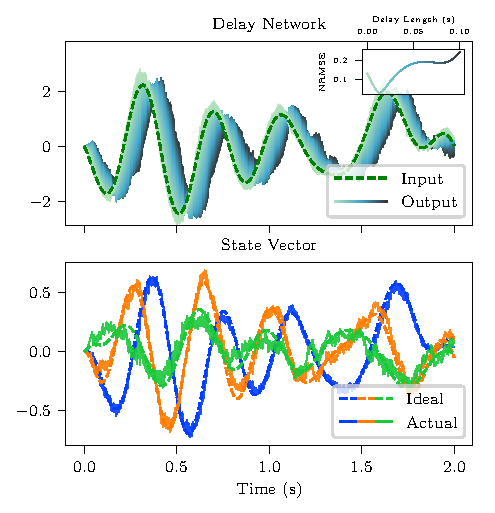
\includegraphics[width=\linewidth]{dn-braindrop}
    \caption{Braindrop Chip}
    \label{fig:dn-braindrop}
  \end{subfigure}%
  \begin{subfigure}{.5\textwidth}
    \centering
    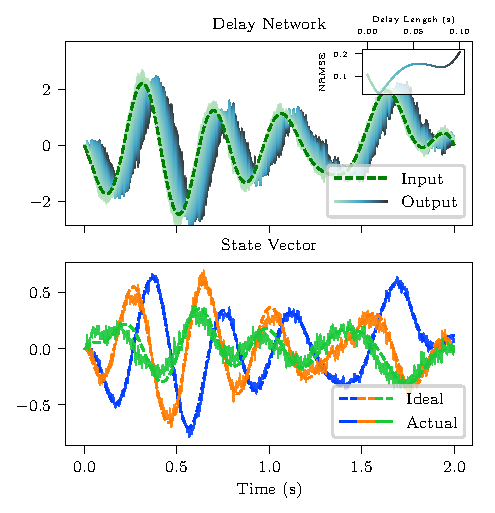
\includegraphics[width=\linewidth]{dn-loihi}
    \caption{Loihi Emulator}
    \label{fig:dn-loihi}
  \end{subfigure}
  \begin{subfigure}{\textwidth}
    \centering
    \vspace{2em}
    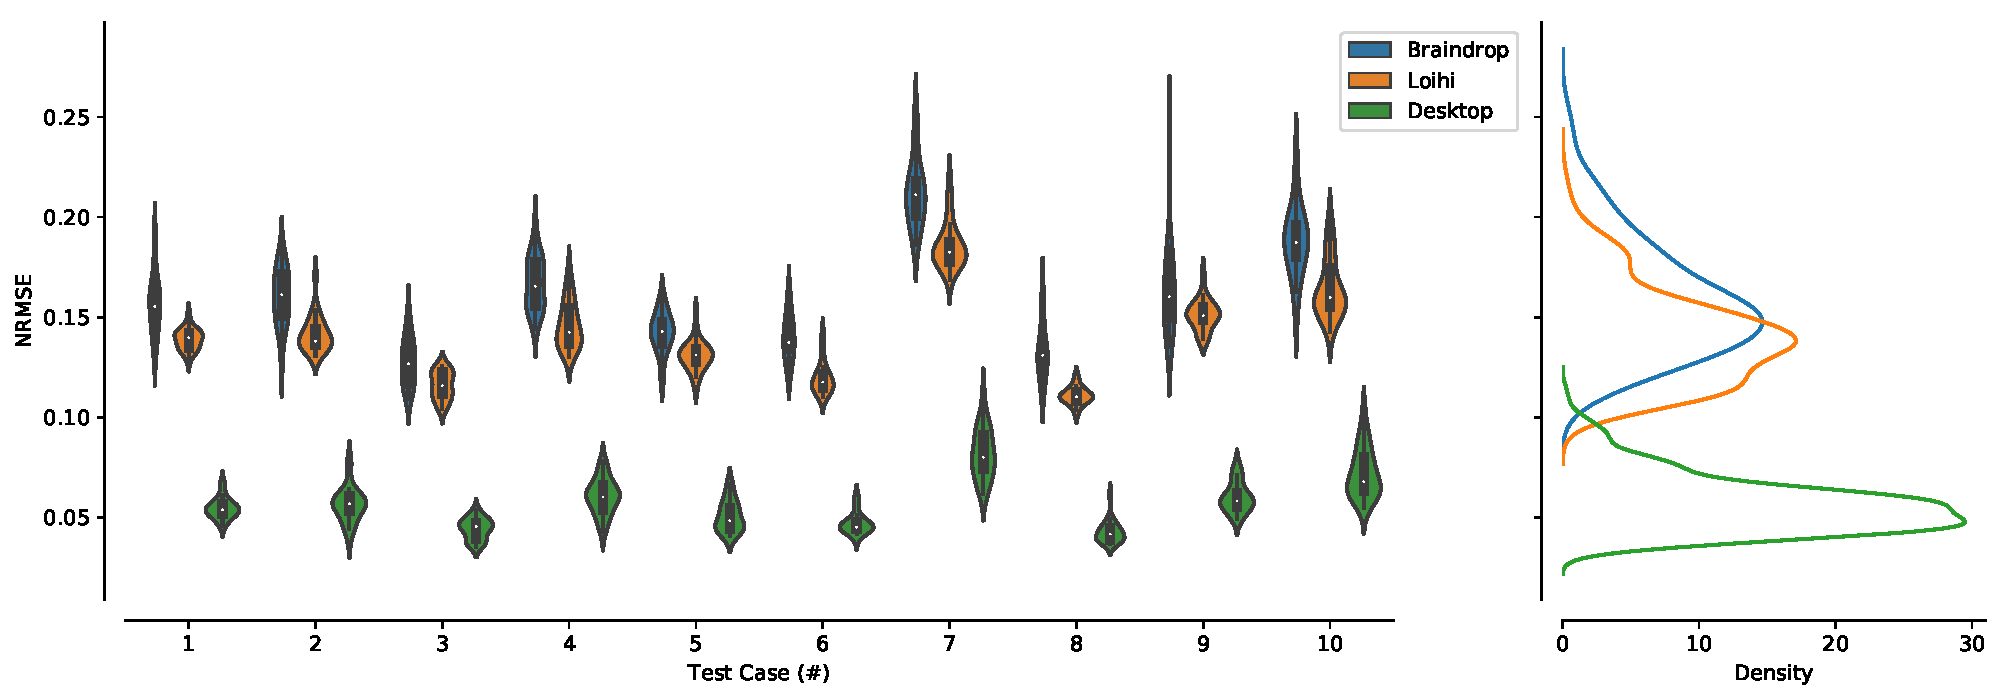
\includegraphics[width=\linewidth]{dn-trials}
    \caption{Overall Error}
    \label{fig:dn-trials}
  \end{subfigure}
  \caption{ \label{fig:dn-neuromorphic}
    Delay Network~(DN; $q=3$, $\theta=100$\,ms; chapter~\ref{chapt:delays}) running on state-of-the-art neuromorphic hardware.
    (a)~Braindrop implementation, reproduced from \citet[][Figure~16]{braindrop2019}. 
    (b)~Loihi Emulator (v0.4.0) implementation.
    (c)~Overall error~(NRMSE) for Braindrop, Loihi, and a standard desktop CPU, across 10 test cases, with 25 randomly initialized network configurations per test case.
    The simulations shown in (a) and (b) correspond to a randomly chosen trial from the first test case in (c).
    See text for details.
  }
\end{figure}


We now instantiate the same Delay Network~(DN) from chapter~\ref{chapt:delays} on state-of-the-art neuromorphic hardware (see Figure~\ref{fig:dn-neuromorphic}).
This system may be conceptualized as an entirely different kind of memory that persists not the sum of the input signal, but finite windows of input history.
In other words, the DN ``buffers'' a sliding window of the input, which enables the computation of arbitrary nonlinear transformations across the window.
This can be used as a basic building block for working memory models that must represent not only \emph{what} has occurred, but also \emph{when} it has occurred in relation to everything else.

To implement the DN, three pools, each containing $128$ spiking neurons, are recurrently coupled to each other (and to themselves), and trained to optimally buffer a white-noise test signal---band-limited to $3$\,Hz---across a $100$\,ms sliding time-window.
Output spikes are filtered using a lowpass synapse with $\tau = 20$\,ms, and weighted to decode both the state-vector and the window of history.
On Braindrop~(see Figure~\ref{fig:dn-neuromorphic}~(a), reproduced from \citet[][Figure~16]{braindrop2019}), the chip is configured to use the default distribution of synaptic time-constants (mean $\tau \approx 18$\,ms).
\TODO{Grab and plot the distribution from the calibration data using the mapped xy coordinates for the 3 ensembles.}
On Loihi~(see Figure~\ref{fig:dn-neuromorphic}~(b)), performance is maximized by using all-to-all weight matrices, and setting the recurrent time-constant to $\tau=10$\,ms.
We also compare this to the reference Nengo simulator ($\tau=10$\,ms) running on a conventional desktop CPU to obtain a baseline level of performance.
The overall error, reported as bootstrapped 95\% confidence intervals across $10 \times 25$~trials, is
[0.156,~0.163] for Braindrop,
[0.146, 0.153] for Loihi (compared to [0.145, 0.151] for the emulator), and
[0.055,~0.059] for the CPU (see Figure~\ref{fig:dn-neuromorphic}~(c)).
